% !TEX TS-program = xepythontex



\documentclass[10pt,envcountsect,spanish]{beamer}


\newif\ifnotas
\notasfalse% Para no mostrar los globos
\notastrue % Para  mostrar los globos

\input ../preambulo.tex


\fvset{frame=leftline, vspace=0pt, fontsize=\small, xleftmargin=.4in, breaklines}


%································ TITULO, AUTOR, ETC
\title{Tipos de Datos Abstractos Con Orden Lineal}
\subtitle{Tecnología de la Programación}


\author[L. Daniel Hernández]{L. Daniel Hernández $<ldaniel@um.es>$}

\institute[ldaniel@um.es]{Dpto. Ingeniería de la Información  y las Comunicaciones\\ Universidad de Murcia\\ 4 de octubre de 2023 \\\,\\\hrule} %	 \\ \today\\ \hrule}


\date[ldaniel@um.es]{ 
\vskip 1.25cm
%\vskip -1.25cm
%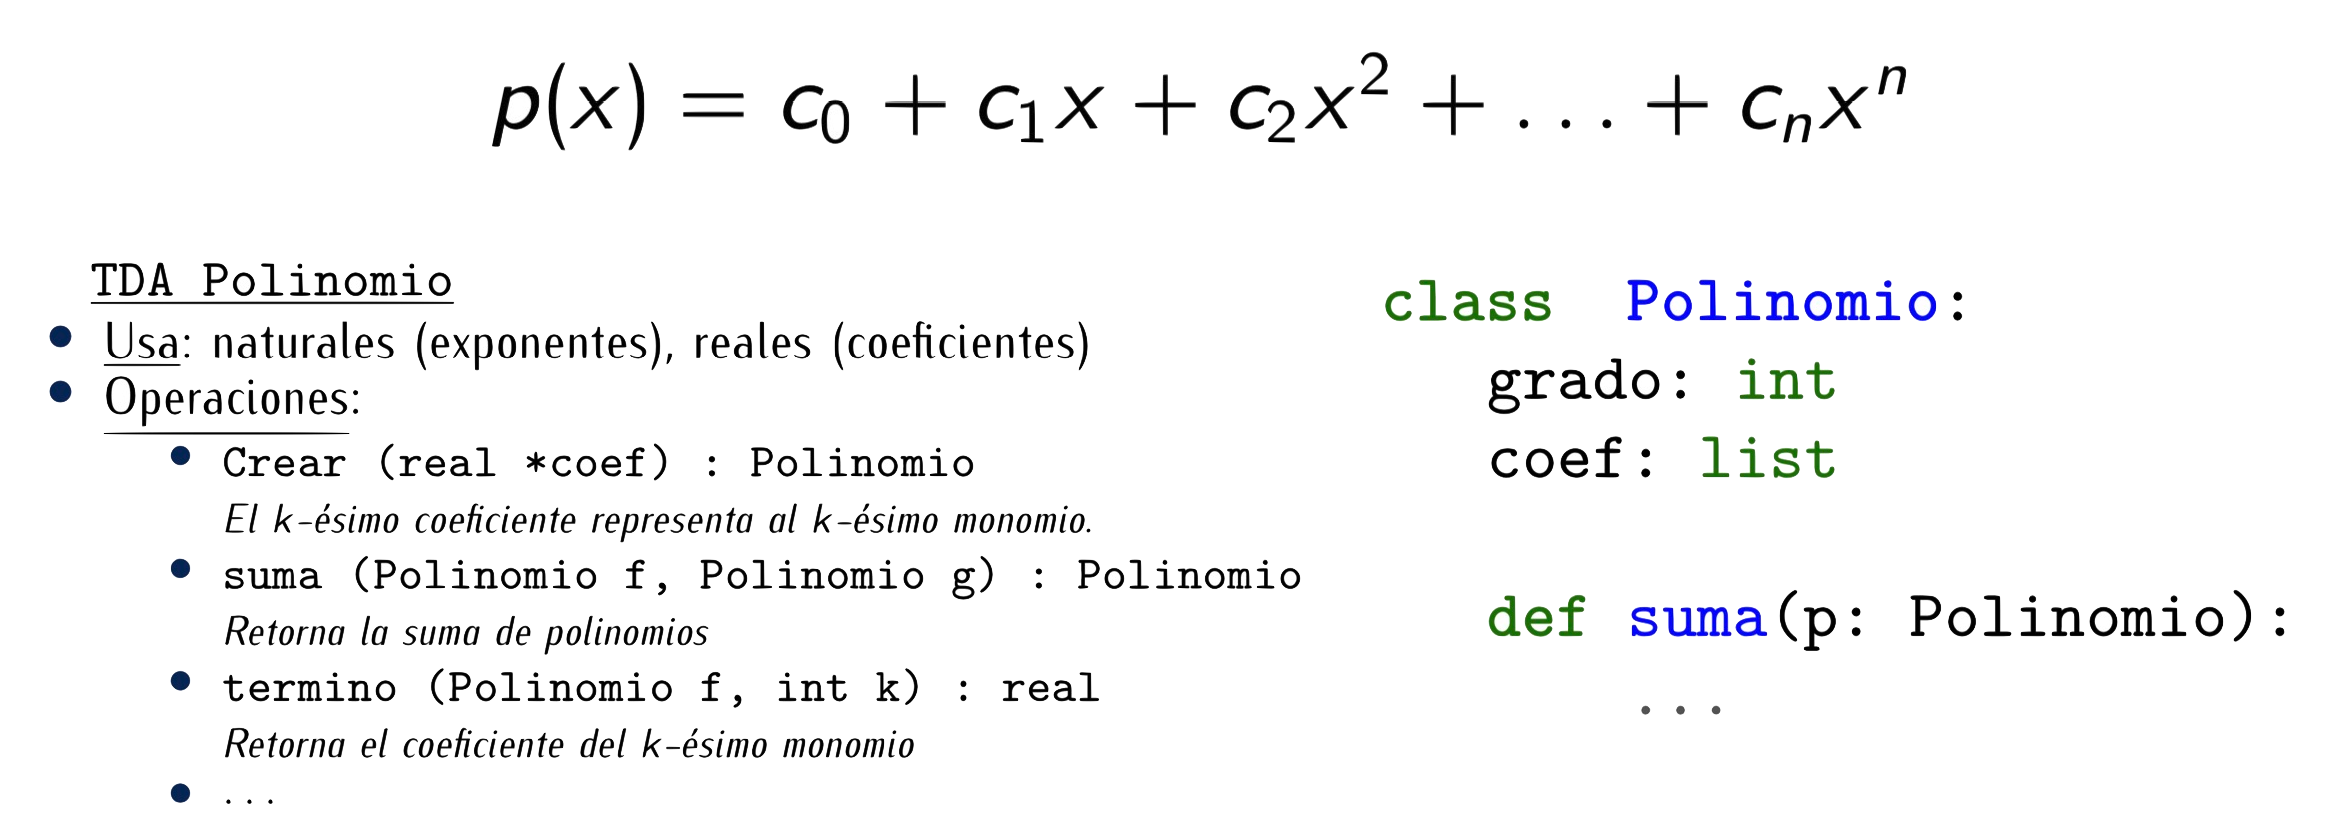
\includegraphics[width=.8\textwidth, height=.18\textheight]{fig/polinomio}
}

\graphicspath{{img/}}



%%%%%%%%%%%%%%%%%%%%%%%%%%%%%%%%%%
%%%%%%%%%%%%%%%%%%%%%%%%%%%%%%%%%%
%%%%%%%%%%%%%%%%%%%%%%%%%%%%%%%%%%
%%%%%%%%%%%%%%%%%%%%%%%%%%%%%%%%%%

%https://es.overleaf.com/learn/how-to/Writing_Markdown_in_LaTeX_Documents
\usepackage[hashEnumerators]{markdown}


%%%%%%%%%%%%%%%%%%%%%%%%%%%%%%%%%%
%%%%%%%%%%%%%%%%%%%%%%%%%%%%%%%%%%
%%%%%%%%%%%%%%%%%%%%%%%%%%%%%%%%%%
%%%%%%%%%%%%%%%%%%%%%%%%%%%%%%%%%%
\begin{document}

%\pgfdeclareimage[height=1cm]{logo}{logo.png}
%\logo{\pgfuseimage{logo}}



%--------------------------------------------------------------------------------
{\usebackgroundtemplate{%
  \includegraphics[width=\paperwidth,height=\paperheight]{../img/fondoUMUCompleto}}
\begin{frame}[b]
	\maketitle

\begin{tikzpicture}[overlay, remember picture]
\node[anchor=south west, %anchor is bottom left corner of the graphic
      xshift=.2\textwidth, %shifting around
      yshift=0.7cm] 
     at (current page.south west) %left bottom corner of the page
     {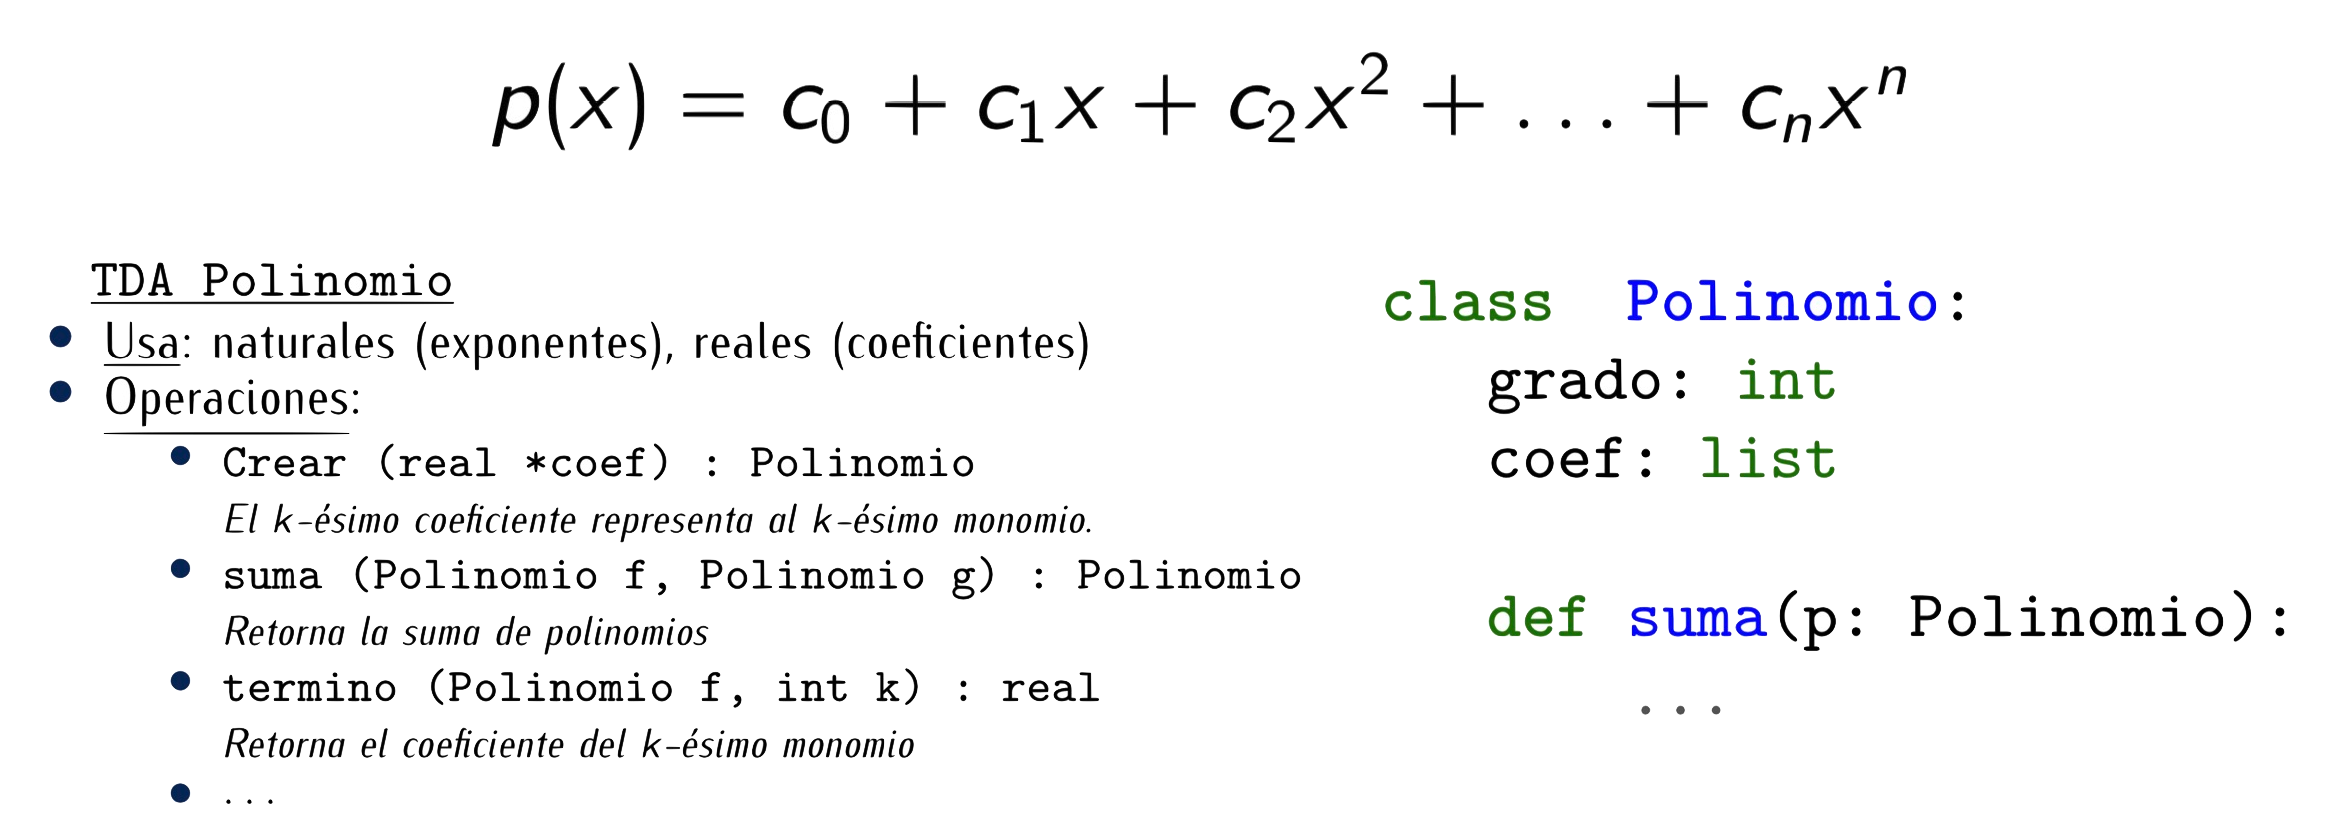
\includegraphics[width=.8\textwidth, height=.3\textheight]{fig/polinomio}}; 
\end{tikzpicture}
	
\end{frame}			% Transparencia: Título
}



%--------------------------------------------------------------------------------
%%%%%%%%%%%%%%%%%%%%%%%%%%%%%%%%%%
%%%%%%%%%%%%%%%%%%%%%%%%%%%%%%%%%%
\begin{frame}{Índice de Contenidos}\tableofcontents \end{frame}


%%%%%%%%%%%%%%%%%%%%%%%%%%%%%%%%%%%%%
%%%%%%%%%%%%%%%  SECTION   %%%%%%%%%%%%%%%
%%%%%%%%%%%%%%%%%%%%%%%%%%%%%%%%%%%%%
\section{TDAs con Orden Lineal}


%%%%%%%%%%%%%%%%%%%%%%%%%%%%%%%%%%
%%%%%%%%%%%%%%%%%%%%%%%%%%%%%%%%%%
\begin{frame}{Qué son los TDAs sin relación de orden}

\begin{itemize}%\setlength{\itemsep}{0mm}

\item Los TDA con \key{ordenación lineal} son aquellos que contienen a un conjunto de objetos pero donde cada objeto tiene exactamente un predecesor inmediato o un sucesor inmediato. 

\item Destacan el primer objeto (que no tiene predecesor) y el último objeto (que no tiene sucesor). 

\item \textbf{Matemáticamente} quedan definidos mediante una relación binaria $a\preceq b$, que será una ordenación lineal sii cumple las siguientes propiedades:
\begin{description}
\item[Completa]  o total. $\forall \; a, b$, o bien $a\preceq b$ o bien $b\preceq a$,
\item[Transitiva.] si $a\preceq b$ y $b\preceq c$, esto implica que $a\preceq c$, y
\item[Antisimétrica.] Si se cumple   $a\preceq b$ y $b\preceq a$, se sigue que $a = b$
\end{description}


\item \key{Las operaciones} que se pueden lleva a cabo en este tipo de contenedores son:
\begin{itemize}
\item \textbf{Acceder} al k-ésimo objeto del orden. En particular, al primer o último objeto en el orden lineal,
\item \textbf{Recorrer} todos los objetos del contenedor en dicho orden.
\item \textbf{Dado un objeto} $a$ que puede, o no,  estar en el contenedor, 
	\begin{itemize}
	\item \textbf{buscar} el objeto predecesor inmediato o el sucesor inmediato en el contenedor.
	\item \textbf{contar} todos los objetos que le preceden o todos los que le suceden.
	\end{itemize}
\item \textbf{Inserta} un nuevo objeto o reemplazar el objeto en la k-ésima posición,
\item Dada una referencia al k-ésimo objeto, \textbf{insertar} un nuevo objeto antes o después de ese objeto; o eliminar el objeto antes o después del k-ésimo objeto.
\end{itemize}


\end{itemize}

\end{frame}



%%%%%%%%%%%%%%%%%%%%%%%%%%%%%%%%%%%%%
%%%%%%%%%%%%%%%  SECTION   %%%%%%%%%%%%%%%
%%%%%%%%%%%%%%%%%%%%%%%%%%%%%%%%%%%%%
\section{Listas}

%%%%%%%%%%%%%%%%%%%%%%%%%%%%%%%%%%
%%%%%%%%%%%%%%%%%%%%%%%%%%%%%%%%%%
\begin{frame}[allowframebreaks]{Listas -}

\begin{itemize}
\item La \key{lista abstracta} se define para objetos que se quieren ordenar explícitamente. Hay un primer elemento que se coloca al inicio del contenedor y un último elemento que  está al final de la lista. Los elementos centrales se colocan de acuerdo al orden lineal definido.

\item Operaciones
\begin{itemize}
\item \cmn{List(): Lista}. Crea una nueva lista, inicialmente vacía.


\item \cmn{len(): int}. Retorna la longitud o número de elementos en la lista.

Para una lista cualquiera $<a_0, a_1, \ldots, a_{n-1}>$ retornará el valor $n$.

\item \cmn{contains(value): bool}. Indica si el valor \cmn{value} se encuentra na la lista.


\item \cmn{getItem(pos): value}. Retorna el elemento o valor almacenado en la posición \cmn{pos}. 

Para una lista cualquiera $<a_0, \ldots, a_{pos}, \ldots, a_{n-1}>$ retornará el valor $a_{pos}$.


\item \cmn{setItem(pos, value): None}. Sustituye el \cmn{pos}-ésimo valor de la lista por \cmn{value}. 

Para una lista cualquiera $<a_0, \ldots, a_{pos}, \ldots, a_{n-1}>$ se modificará la lista a la secuencia $<a_0, \ldots, value, \ldots, a_{n-1}>$.

\item \cmn{insertItem(pos, value): None}. Inserta el  \cmn{pos}-ésimo valor de la lista por \cmn{value}. 

Para una lista cualquiera $<a_0, \ldots, a_{pos}, \ldots, a_{n-1}>$ se modificará la lista a la secuencia $<a_0, \ldots, value, a_{pos}, \ldots, a_{n-1}>$.


\item \cmn{removeItem(pos): None}. Elimina el elemento de la posición dada, si existe en la lista.

Dada una lista cualquiera $<a_0, \ldots, a_{pos}, \ldots, a_{n-1}>$ se modificará la lista a la secuencia $<a_0, \ldots, a_{pos-1},a_{pos+1},\ldots, a_{n-1}>$.


\item \cmn{clear(): None}. Limpia la lista. Se convierte en una lista vacía.

Modifica cualquier lista a la lista  $<>$.

\item \cmn{isEmpty(): bool}. Indica si la lista está vacía o no.

\item \cmn{first(): pos}. Retorna la posición del primer elemento de la lista. Si la lista está vacía retornará  \cmn{last()}

Dada una lista  $<a_0, \ldots, a_{pos}, \ldots, a_{n-1}>$ se retornará la posición donde se localiza $a_0$.

\item \cmn{last(): pos}. Retorna la posición del último elemento de la lista. Si la lista está vacía retornará  \cmn{last()}

Dada una lista  $<a_0, \ldots, a_{pos}, \ldots, a_{n-1}>$ se retornará la posición donde se localiza $a_{n-1}$.

\item \cmn{next(pos): pos}. Retorna la posición del elemento siguiente al elemento de la posición dada.

Dada una lista retornará la posición donde se localiza el elemento $a_{pos+1}$.

\item \cmn{previous(pos): pos}. Retorna la posición del elemento anterior al elemento de la posición dada.

Dada una lista retornará la posición donde se localiza el elemento $a_{pos-1}$.


\item \cmn{iterator(): Lista}: Crea y retorna un iterador para la lista.
\end{itemize}

\end{itemize}

\end{frame}


%%%%%%%%%%%%%%%%%%%%%%%%%%%%%%%%%%%%%
%%%%%%%%%%%%%%%  SECTION   %%%%%%%%%%%%%%%
%%%%%%%%%%%%%%%%%%%%%%%%%%%%%%%%%%%%%
\subsection{Implementación de Listas}


%%%%%%%%%%%%%%%%%%%%%%%%%%%%%%%%%%%%%
%%%%%%%%%%%%%%%  SECTION   %%%%%%%%%%%%%%%
%%%%%%%%%%%%%%%%%%%%%%%%%%%%%%%%%%%%%
\subsubsection{Arrays}

%%%%%%%%%%%%%%%%%%%%%%%%%%%%%%%%%%
%%%%%%%%%%%%%%%%%%%%%%%%%%%%%%%%%%
\begin{frame}[fragile]{Implementación de Listas: Arrays}

\begin{itemize}
\item \key{Arrays}: cada elemento del array contiene un elemento de la lista, indexados/ordenados de acuerdo al orden lineal.

\item Un array 'puro' presenta inconvenientes de gestión de memoria.
\item Alternativamente se usa esta representación.

\begin{pyverbatim}
struct rep
   int pos; # la primera posición vacía
   int len; # longitud de la lista
   object[] list;  # la lista
\end{pyverbatim}


\begin{itemize}
\item La \key{función de abstracción}:
$
Abst: \mbox{\textbf{rep}} \longrightarrow {\cal A}
$
la definiremos como

\centerline{\ttfamily{$Abst($r$) = <$r.list[0], r.list[1], $\ldots$, r.list[len-1]$>$}}

\item El \key{invariante de la representación} 
$I: \mbox{\textbf{rep}} \longrightarrow \mathbb{B}$,  lo definimos de esta manera:
$$I( \text{r} ) =
\left\{
\begin{array}{l}
\forall p, p < \text{r.pos} \Rightarrow \text{r.list[r.p]} \not= NULL\ and \\
\forall p, p \geq \text{r.pos} \Rightarrow \text{r.list[r.p]} = NULL \ and \\
\text{r.list} \not= NULL \ (\text{r.len} > 0)
\end{array}
\right.
$$


Con este invariante hay una lista que no se puede representar ¿cuál?

\end{itemize}

\end{itemize}

\end{frame}




%%%%%%%%%%%%%%%%%%%%%%%%%%%%%%%%%%%%%
%%%%%%%%%%%%%%%  SECTION   %%%%%%%%%%%%%%%
%%%%%%%%%%%%%%%%%%%%%%%%%%%%%%%%%%%%%
\subsubsection{Nodos}


%%%%%%%%%%%%%%%%%%%%%%%%%%%%%%%%%%
%%%%%%%%%%%%%%%%%%%%%%%%%%%%%%%%%%
\begin{frame}[fragile]{Implementación de Listas: Nodos}

\begin{itemize}
\item \key{Nodo}: Estructura con 1 valor y 1 o más referencias a nodos.

\item \key{Nodo Simple}: Estructura con 1 valor y 1 referencia.


\item \key{Estructura enlazada}: Estructura de datos formada por nodos.

\item \key{Estructura simplemente enlazada}: Estructura enlazada formada por nodos simples.

\item Una lista se puede representar mediante una estructura simplemente enlazada.

\item \key{Función de abstracción:} $Abst: \mbox{\textbf{node}} \longrightarrow {\cal A}$

\centerline{\ttfamily{$Abst($r$) = <$r.valor, r.next.valor, $\ldots$, r.next.\ldots.next.valor$>$}}

\item El \key{invariante de la representación} 
$I: \mbox{\textbf{node}} \longrightarrow \mathbb{B}$, que se define así:
\begin{itemize}
\item Consta de una colección de nodos donde cada uno tiene una referencia a otro nodo (cuyo campo llamaremos \cmn{siguiente} o \cmn{next}).

\item En dos nodos diferentes la referencia \cmn{next} son diferentes.

\item Se tiene una variable externa que hace referencia a aquel nodo tal que a partir de él se puede recorrer todos los elementos de la lista pasando por la referencia de \cmn{next} de cada uno.
\end{itemize}

\end{itemize}

\end{frame}





%%%%%%%%%%%%%%%%%%%%%%%%%%%%%%%%%%
%%%%%%%%%%%%%%%%%%%%%%%%%%%%%%%%%%
\begin{frame}[fragile, allowframebreaks]{Operaciones básicas con Estructuras enlazadas -}

\begin{enumerate}
\item \key{Recorrer los nodos.} 

\begin{pyverbatim}
actual = primer nodo de la lista
mientras actual is not None:
  trabajar con actual
  actual = actual.next
\end{pyverbatim}

\

\


\item \key{Buscar un nodo.}

\begin{pyverbatim}
actual = primer nodo de la lista
mientras actual is not None y actual.value != target:
  actual = actual.next
trabajar con actual
\end{pyverbatim}

\framebreak 

\item \key{Añadir un nodo como siguiente de otro.} 

\begin{pyverbatim}
pos = referencia # Pondremos uno delante de este
nuevo_nodo = Node(VALUE)
nuevo_nodo = pos.next
pos.next = nuevo_nodo
\end{pyverbatim}

\

\

\item \key{Eliminar el nodo siguiente de otro.} 

\begin{pyverbatim}
pos = referencia # Eliminaremos el siguiente a este
borrar = pos.next
pos.next = borrar.next
gc.collect()
\end{pyverbatim}

\end{enumerate}

\end{frame}





%%%%%%%%%%%%%%%%%%%%%%%%%%%%%%%%%%
%%%%%%%%%%%%%%%%%%%%%%%%%%%%%%%%%%
\begin{frame}[fragile, allowframebreaks]{Modificaciones sobre una Estructuras Enlazada Simple}

\begin{itemize}
\item Considerar un \key{nodo cabecera}. El nodo cabecera NO forma parte de la lista, pero apunta al primer elemento de la lista.

\begin{pyverbatim}
struct node  # Estructura del nodo
    TD valor
    node next

struct List  # Lista simplemente enlazada
  # Descomentar el adecuado, en su caso:
  # node head # Apunta a una cabecera
  # node list # Apunta al primer elemento de la lista
\end{pyverbatim}

\

\


\item Para recorrer la lista desde cualquier punto, considerar \key{listas circulares}.


\framebreak


\item Si se quiere añadir \key{elementos al final}, tener un campo \texttt{ultimo} al último elemento de la lista.

\begin{pyverbatim}
struct node  # Estructura del nodo
    TD valor
    node next

struct List  # Lista simplemente enlazada
  node list
  node last # con referencia al último elemento de la lista
\end{pyverbatim}


\

\




\item Si hay que hacer muchos recorridos, considerar una \key{lista doblemente enlazada}.


\begin{pyverbatim}
struct node 
   TD valor
   node next
   node previous
\end{pyverbatim}


\end{itemize}

\end{frame}





%%%%%%%%%%%%%%%%%%%%%%%%%%%%%%%%%%%%%
%%%%%%%%%%%%%%%  SECTION   %%%%%%%%%%%%%%%
%%%%%%%%%%%%%%%%%%%%%%%%%%%%%%%%%%%%%
\subsection{Búsqueda y Ordenación en Listas}


%%%%%%%%%%%%%%%%%%%%%%%%%%%%%%%%%%%%%
%%%%%%%%%%%%%%%  SECTION   %%%%%%%%%%%%%%%
%%%%%%%%%%%%%%%%%%%%%%%%%%%%%%%%%%%%%
\subsubsection{Búsqueda}

%%%%%%%%%%%%%%%%%%%%%%%%%%%%%%%%%%
%%%%%%%%%%%%%%%%%%%%%%%%%%%%%%%%%%
\begin{frame}{Búsqueda en listas}

\begin{itemize}
\item Un \concepto{algoritmo de búsqueda} es aquel que está diseñado para localizar un elemento con ciertas propiedades dentro de una estructura de datos. Por ejemplo, encontrar el registro correspondiente a cierta canción en un array de canciones.


\item Dependiendo de cómo se encuentren ordenados los elementos de la colección, podemos aplicar uno de los dos siguientes algoritmos: 

\begin{itemize}
\item o \key{búsqueda secuencial}, cuando los elementos de la colección no están ordenados
\item o \key{búsqueda binaria}, para cuando los elementos están ordenados.
\end{itemize}

\end{itemize}

\end{frame}




%%%%%%%%%%%%%%%%%%%%%%%%%%%%%%%%%%%%%
%%%%%%%%%%%%%%%  SECTION   %%%%%%%%%%%%%%%
%%%%%%%%%%%%%%%%%%%%%%%%%%%%%%%%%%%%%
\subsubsection{Ordenación}

%%%%%%%%%%%%%%%%%%%%%%%%%%%%%%%%%%
%%%%%%%%%%%%%%%%%%%%%%%%%%%%%%%%%%
\begin{frame}[fragile]{Ordenación en listas}

\begin{itemize}
\item Un \concepto{algoritmo de ordenación} u ordenamiento es aquel que está diseñado para ordenar los elementos de una lista. 

\item Será necesario aclarar qué se entiende por la expresión \cm{vec[pos1]$<$vec[pos2]}:  operación construida por el programador.

\item Algoritmos conocidos de ordenación, y que se consideran \textbf{ya aprendidos}.

\begin{itemize}
\item \key{Ordenación de Burbuja.} Se revisa la lista una y otra vez, intercambiando los valores de dos posiciones consecutivas si dichos valores no están ordenados.

\begin{verbatim}
4 5 3 2 (swap)
4 3 5 2
4 3 2 5
\end{verbatim}

\item \key{Ordenación por Selección.} Selecciona el elemento más pequeño de la lista y lo coloca en su posición. Después busca el siguiente más pequeño de entre el resto de la lista y lo coloca en su sitio, y así se repite una y otra vez.


\begin{verbatim}
4 5 3 2 (min = 2)
2 3 5 4
\end{verbatim}


\item \key{Ordenación por inserción.} En el paso k, se considera el valor de la posición k y el anterior (inicialmente en la posición k-1). Mientras que el anterior sea menor que el valor se intercambian los valores (actualizando en cada bucle el valor de anterior).

\begin{verbatim}
4 5 3 2 (k=2)
3 4 5 2
\end{verbatim}

\end{itemize}


\end{itemize}

\end{frame}






%%%%%%%%%%%%%%%%%%%%%%%%%%%%%%%%%%%%%
%%%%%%%%%%%%%%%  SECTION   %%%%%%%%%%%%%%%
%%%%%%%%%%%%%%%%%%%%%%%%%%%%%%%%%%%%%
\subsubsection{Ordenación por }

%%%%%%%%%%%%%%%%%%%%%%%%%%%%%%%%%%
%%%%%%%%%%%%%%%%%%%%%%%%%%%%%%%%%%
\begin{frame}[fragile]{Ordenación por Casilleros y por Mezclas}

\begin{itemize}
\item \concepto{Ordenación por Casilleros.}

\begin{enumerate}
\item Crear una colección de casilleros vacíos, que ya está ``ordenados'' entre sí.
\item Colocar cada elemento a ordenar de la lista en un único casillero.
\item Ordenar los elementos de cada casillero según el algoritmo que se considere más adecuado.
\item Devolver los elementos de cada casillero ``concatenados''.
\end{enumerate}



\item \concepto{Ordenación por Mezclas.} Dada una lista, 


\begin{enumerate}
\item Si la lista tienen un elemento retornar la lista.
\item En otro caso, dividir (recursivamente) la lista en dos partes 'simétricas'.
\item Mezclar las dos listas:
	\begin{itemize}
	\item Mientras que alguna de las listas tenga elementos hacer:
		\begin{enumerate}
		\item Se comparan los dos primeros elementos de la lista y se quita el más pequeño.
		\item El más pequeño se añade a la lista solución.
		\end{enumerate}
	\item Añadir los elementos de la lista no vacía a la lista solución.
	\end{itemize}
\item Retornar la lista solución.
\end{enumerate}

\end{itemize}

\end{frame}






%%%%%%%%%%%%%%%%%%%%%%%%%%%%%%%%%%%%%
%%%%%%%%%%%%%%%  SECTION   %%%%%%%%%%%%%%%
%%%%%%%%%%%%%%%%%%%%%%%%%%%%%%%%%%%%%
\section{Pilas}

%%%%%%%%%%%%%%%%%%%%%%%%%%%%%%%%%%
%%%%%%%%%%%%%%%%%%%%%%%%%%%%%%%%%%
\begin{frame}{Pilas}

\begin{itemize}
\item Una \key{pila} es una lista con el criterio LIFO.

\item Operaciones
\begin{itemize}
\item \cmn{Stack() : Stack}. Crea una nueva pila, inicialmente vacía.

\item \cmn{peek() : value}. Retorna el valor del tope. También se suele usar la signatura \cm[black]{top() : value}.

Para una pila  $<a_0, a_1, \ldots,>$ retornará el valor $a_0$.

\item \cmn{pop() : value}. Retorna el valor del tope y además borra el primer nodo de la pila.

Para una pila  $<a_0, a_1, a_2, \ldots,>$ retornará el valor $a_0$ y la nueva pila es  $<a_1, a_2, \ldots,>$.


\item \cmn{push(value) : None}. Inserta un nuevo nodo en el tope de la lista. 

Para una pila  $<a_0, a_1, a_2, \ldots,>$ y un valor $value$ la pila se modifica para conseguir la pila $<value, a_0, a_1, a_2, \ldots,>$.


\item \cmn{len() : int}. Retorna el número de elementos de la pila.

\item \cmn{isEmpty() : Bool}. Indica si la pila está vacía o no.

\item \cmn{clear() : None}. Limpia la pila y la deja sin elementos.

\end{itemize}

\item MUY IMPORTANTE: No se puede acceder directamente a ningún elemento central.


\end{itemize}

\end{frame}







%%%%%%%%%%%%%%%%%%%%%%%%%%%%%%%%%%%%%
%%%%%%%%%%%%%%%  SECTION   %%%%%%%%%%%%%%%
%%%%%%%%%%%%%%%%%%%%%%%%%%%%%%%%%%%%%
\section{Colas y Colas de Prioridad}

%%%%%%%%%%%%%%%%%%%%%%%%%%%%%%%%%%
%%%%%%%%%%%%%%%%%%%%%%%%%%%%%%%%%%
\begin{frame}{Colas y Colas de Prioridad}

\begin{itemize}
\item Una \key{cola} es una lista con el criterio FIFO.

\item Operaciones
\begin{itemize}
\item \cmn{Queue() : Queue}. Crea una nueva cola, inicialmente vacía.

\item \cmn{peek() : value}. Retorna el valor del primer elemento de la lista, pero no lo borra.  También es usual esta signatura \cm[black]{front() : value}.

\item \cmn{dequeue() : value}. Retorna el primer elemento de la cola borrandolo de la cola. También es usual esta signatura  \cm[black]{top() : value}.

Para la cola  $<a_0, a_1, \ldots,>$ retornará el valor $a_0$.
Se genera un error si la cola está vacía.

\item \cmn{enqueue(value) : None}.
Añade un nuevo elemento al final de la cola

Para la cola  $<a_0, a_1, \ldots, a_{n-1}>$ 
se modificará a la lista $<a_0, a_1, \ldots, a_{n-1}, value>$ 

\item \cmn{len() : int}. Retorna el número de elementos de la cola.

\item \cmn{isEmpty() : Bool}. Indica si la cola está vacía o no.

\item \cmn{clear() : None}. Limpia la cola y la deja sin elementos.

\end{itemize}

\item Una \key{cola de prioridad} es una cola pero que el encolar a un elemento nuevo lo coloca en la posición que le corresponda en el orden. Las demás operaciones son iguales.


\item MUY IMPORTANTE: No se puede acceder directamente a ningún elemento central.

Acceder directamente es suspender el examen.

\end{itemize}

\end{frame}






%%%%%%%%%%%%%%%%%%%%%%%%%%%%%%%%%%%%%
%%%%%%%%%%%%%%%  SECTION   %%%%%%%%%%%%%%%
%%%%%%%%%%%%%%%%%%%%%%%%%%%%%%%%%%%%%
\section{Ordenación usando Pilas y Colas}

%%%%%%%%%%%%%%%%%%%%%%%%%%%%%%%%%%
%%%%%%%%%%%%%%%%%%%%%%%%%%%%%%%%%%
\begin{frame}[fragile]{Ordenación}

\begin{pyverbatim}[][frame=single]
def search(initial, goal_test, successors):
  # Nodo = {estado, nodo_padre}
  
  frontera = [Nodo(initial, None)]  # LISTA de nodos que 
                    # contienen a los estados a expandir
  explorados = {initial} # CONJUNTO de estados analizados
  
  mientras que la frontera no esté vacía:
     nodo_actual = extraer un nodo de frontera (y borrarlo) # PILA, COLA (de prioridad)
     estado_actual = estado del nodo_actual
     si goal_test(estado_actual):
         retornar camino solución para el nodo_actual
     para cada estado de successors(estado_actual):
         si estado está en explorados:
             pasar al siguiente estado
         añadir estado a explorados
         añadir el nodo(estado, nodo_actual) a frontera
  retornar None
\end{pyverbatim}

\end{frame}






\end{document}




%%%%%%%%%%%%%%%%%%%%%%%%%%%%%%%%%%%%%
%%%%%%%%%%%%%%%  SECTION   %%%%%%%%%%%%%%%
%%%%%%%%%%%%%%%%%%%%%%%%%%%%%%%%%%%%%
\section{Set}

%%%%%%%%%%%%%%%%%%%%%%%%%%%%%%%%%%
%%%%%%%%%%%%%%%%%%%%%%%%%%%%%%%%%%
\begin{frame}[allowframebreaks]{Set -}


\begin{itemize}%\setlength{\itemsep}{0mm} \footnotesize
\item Un Bag  donde \textbf{no se permite} la repetición de elementos. 

\item Operaciones:
\begin{itemize}
\item \cmn{Set(): Set}. Crea un nuevo conjunto, \textit{set}, inicialmente vacío.

\item \cmn{len(): int}. Retorna el número de elementos en el conjunto.

Para una lista cualquiera $<a_0, a_1, \ldots, a_{n-1}>$ retornará el valor $n$.

\item \cmn{contains(element): bool}. Indica si el elemento \cmn{element} se encuentra en el conjunto. Retorna \cm{True} si está contenido y \cm{False} si no está contenido.

\item \cmn{add(element): None}. Modifica el conjunto añadiendo  el elemento \cmn{element} al conjunto.

\item \cmn{remove(element): None}. Elimina el elemento \cmn{element} del conjunto. Lanza un error si el elemento no existe.


\item \cmn{iterator(): IteratorSet}: Crea y retorna un iterador para el conjunto.


\item \cmn{isSubsetOf(setB): bool}. Determina si un conjunto es subconjunto del conjunto dado. 

Un conjunto A es subconjunto de B si todos los elementos de A están en B.

\item \cmn{equal(setB): bool}. Determina si el conjunto es igual al conjunto dado. 

Dos conjuntos son iguales si ambos contienen el mismo número de elementos y todos los elementos del conjunto está en el conjunto B. Si ambos están vacíos entonces son iguales.


\item \cmn{union(setB): Set}. Retorna un nuevo conjunto que es la unión del conjunto con el conjunto dado.

La unión del conjunto A  con el conjunto de B es un nuevo conjunto que está formado por todos los elementos de A y todos los elementos de B que no están en A.


\item \cmn{difference(setB): Set}.  Retorna un nuevo conjunto que es la diferencia del conjunto con el conjunto dado.

La diferencia del conjunto A  con el conjunto de B es un nuevo conjunto que está formado por todos los elementos de A que no están en B.


\item \cmn{intersect(): Set}.  Retorna un nuevo conjunto que es la intersección del conjunto con el conjunto dado.

La intersección del conjunto A  con el conjunto de B es un nuevo conjunto que está formado por todos los elementos que están en A y también en B.

\end{itemize}

\item Notar que los 6 primeros operadores del TDA Set son análogos a los operadores del TDA Bag. Los restantes son operaciones bien conocidas de los conjuntos matemáticos.


\end{itemize}

\end{frame}




%%%%%%%%%%%%%%%%%%%%%%%%%%%%%%%%%%%%%
%%%%%%%%%%%%%%%  SECTION   %%%%%%%%%%%%%%%
%%%%%%%%%%%%%%%%%%%%%%%%%%%%%%%%%%%%%
\section{Map}

%%%%%%%%%%%%%%%%%%%%%%%%%%%%%%%%%%
%%%%%%%%%%%%%%%%%%%%%%%%%%%%%%%%%%
\begin{frame}{Map}


\begin{itemize}%\setlength{\itemsep}{0mm} \footnotesize
\item Colección de registros no repetidos donde cada uno consta de una clave y un valor. La clave debe ser comparable y es la que se utiliza para poder acceder al valor.

\item Ejemplos: tener las notas de los estudiantes por su identificador de estudiante, los datos fiscales por algún número de identificación, los datos de un conductor por el número de matricula de su vehículo,  etc ... 


\item Operaciones:

\begin{itemize}
\item \cmn{Map(): Map}. Crea un nuevo map vacío.

\item \cmn{len(): int}. Retorna el número de registros clave/valor que existen en el map..

\item \cmn{contains(key): bool}. Indica si la clave \cmn{key} se encuentra en el contenedor. Retorna \cm{True} si la clave está contenida y \cm{False} si no está contenida.


\item \cmn{remove(key): None}. Elimina el registro que tiene como clave el valor \cmn{key}. Lanza un error si el elemento no existe.


\item \cmn{add(key, value): None}. Modifica el map añadiendo el par \cmn{key/value} al contenedor. Si existiera un registro con la clave \cmn{key} se sustituye el par \cmn{key/value} existente por el nuevo par \cmn{key/value}. Retorna \cm{True} si la clave es nueva y \cm{False} si se realiza una sustitución.


\item \cmn{valueOf(key):  TipoValor}.  Retorna el valor asociado a la clave dada. La clave debe de existir en el Map.

\item \cmn{iterator(): IteratorMap}: Crea y retorna un iterador para el conjunto.
\end{itemize}
\end{itemize}

\end{frame}



%%%%%%%%%%%%%%%%%%%%%%%%%%%%%%%%%%%%%
%%%%%%%%%%%%%%%  SECTION   %%%%%%%%%%%%%%%
%%%%%%%%%%%%%%%%%%%%%%%%%%%%%%%%%%%%%
\section{Implementación}


%%%%%%%%%%%%%%%%%%%%%%%%%%%%%%%%%%
%%%%%%%%%%%%%%%%%%%%%%%%%%%%%%%%%%
\begin{frame}[fragile]{Cómo implementar los TDAs sin orden}

\begin{itemize}

\item \key{Estructuras integradas del lenguaje.}

\begin{itemize}
\item Algunas estructuras conocidas son: \cmn{array},  \cmn{list}, \cmn{tuple} y \cmn{dictionary}, \cmn{namedtuple}, \cmn{chainmap}, etc ...

\item Dependerá del lenguaje particular.


\item Python no tiene arrays.
\end{itemize}



\item \key{Estructuras enlazadas.} 

\begin{itemize}
\item Una estructura enlazada es aquella que se construye utilizando como estructura básica un \key{nodo}: 

\begin{pyverbatim}
struct Nodo
   valor: TDA
   referencia1 Nodo
   referencia2 Nodo
   ...
\end{pyverbatim}

\item Es una estructura construida por el programador.

\item Un nodo  sirve para representar muchos conceptos.

Ejemplo: elementos de un conjunto, los de una lista o los vértices de un árbol o un grafo.  

\item Distintos tipos de nodos nos sirve para implementar el mismo concepto de TDA. 

Ejemplo: un conjunto se puede implementar con un una referencia o con dos referencias.
\end{itemize}

\end{itemize}

\end{frame}


%%%%%%%%%%%%%%%%%%%%%%%%%%%%%%%%%%
%%%%%%%%%%%%%%%%%%%%%%%%%%%%%%%%%%
\section{Estructuras útiles de Python}
%%%%%%%%%%%%%%%%%%%%%%%%%%%%%%%%%%
%%%%%%%%%%%%%%%%%%%%%%%%%%%%%%%%%%


\begin{frame}{Estructuras útiles de Python}
%\small 
\begin{itemize}% \setlength{\itemsep}{0mm}
\item Rangos
\item Listas
\item Tuplas
\item Diccionarios
\end{itemize}
\end{frame}

\end{document}

%%%%%%%%%%%%%%%%%%%%%%%%%%%%%%%%%%
%%%%%%%%%%%%%%%%%%%%%%%%%%%%%%%%%%
\subsection{Abstracción de Datos}
%%%%%%%%%%%%%%%%%%%%%%%%%%%%%%%%%%
%%%%%%%%%%%%%%%%%%%%%%%%%%%%%%%%%%
\begin{frame}{Abstracción de Datos}
\begin{itemize}% \setlength{\itemsep}{0mm}
\item Existen 3 tipos (o niveles) de abstracción.
\item \key{Tipos de datos integrados}  (o fundamentales). Son los que ofrecen los lenguajes de programación.

\cm[magenta]{Ejemplo:} En \cm[red]{Python} se distinguen, entre otros\footnote[frame]{\url{https://docs.python.org/es/3/library/stdtypes.html}}:
\begin{itemize}
\item Los tipos de datos simples: numéricos (enteros, reales y complejos) y booleanos.
\item Los tipos de datos compuestos: cadena de caracteres (str), secuencias (rangos, listas y tuplas), mapas (diccionarios), conjuntos.
\end{itemize}


\item \key{Tipos de datos definidos por el usuario} o programador. Son los que pueden diseñar los programadores agrupando todos de datos fundamentales. 

\begin{itemize}
\item array, record, struct, \cm{class}
\end{itemize}

\item \key{Tipos de datos abstractos (TDA).} Construye modelos (matemáticos) usando agrupación de datos.

\begin{itemize}
\item No es lo mismo una estructura de datos formado por dos valores y operar con ellos que trabajar con vectores numéricos 2D con operaciones matemáticas (donde no importa la estructura).
\end{itemize}

\end{itemize}

\end{frame}




%%%%%%%%%%%%%%%%%%%%%%%%%%%%%%%%%%
%%%%%%%%%%%%%%%%%%%%%%%%%%%%%%%%%%
\section{Tipos de Datos Abstractos}
%%%%%%%%%%%%%%%%%%%%%%%%%%%%%%%%%%
%%%%%%%%%%%%%%%%%%%%%%%%%%%%%%%%%%
\begin{frame}{Tipos de Datos Abstractos}

\begin{itemize}
\item  Los \key{Tipos de Datos Abstractos} (TDA) son \textbf{modelos matemáticos} que constan de

\begin{itemize}
\item un nombre publico para 
\item identificar a un conjunto de datos (valores), junto con
\item un conjunto de operaciones bien definidas sobre los datos (como en una estructura algebraica). 
\end{itemize}

\item Como modelo, le es \key{irrelevante} cómo se almacenan o estructuren los datos y cómo se implementan las operaciones.

\item Para todo TDA hemos de abordar \key{tres tareas}: 

\begin{itemize}
\item \textbf{Especificación:} definición del TDA 
\item \textbf{Representación:} estructura con la que representar el TDA.
\item \textbf{Implementación:} cómo implementar la estructura en un lenguaje de programación.
\end{itemize}

\end{itemize}
\end{frame}




%%%%%%%%%%%%%%%%%%%%%%%%%%%%%%%%%%
%%%%%%%%%%%%%%%%%%%%%%%%%%%%%%%%%%
\subsection{Especificación de TDAs}
%%%%%%%%%%%%%%%%%%%%%%%%%%%%%%%%%%
%%%%%%%%%%%%%%%%%%%%%%%%%%%%%%%%%%
\begin{frame}{Especificación de TDAs}

\begin{itemize}
\item La \key{especificación} de un TDA (Datos+Operaciones) se rige por las normas generales de la \textit{\bf Abstracción por Especificación}

\item La especificación consta de \key{tres partes}: nombre y descripción, la definición de los datos y la definición de los operadores.

\item \key{Nombre y descripción.}
\begin{itemize}
\item Se le dará un nombre que identifica al conjunto de datos y las operaciones.
\item Se indicará qué representan.
\end{itemize}


\item \key{Especificación de los datos.}
\begin{itemize}

	
\item Pueden venir dados por reglas.

\unEjemplo Definiciones recursivas (p.e. una lista).


\item Puede usar notaciones matemáticas conocidas.

\unEjemplo Conjuntos conocidos ($\mathbb{N}$, $\mathbb{R}$, ...), conjuntos $\{s_1,s_2,\ldots\}$, intervalos $[a, b]$, expresiones regulares, ... 

\item Nunca se definirá pensando en estructuras concretas de un lenguaje de programación. 

\end{itemize}


\item \key{Especificación de las Operaciones} (abstractas).

\begin{itemize}
\item Se indicará tanto la sintaxis como la semántica de cada una. 
\item Se emplearan las especificaciones de la abstracción procedimental.
\end{itemize}


\item \textbf{IMPORTANTE.} \key{Un TDA define un valor de tipo $T$:} 

\centerline{\it Todos los entes/valores que respondan al TDA $T$ son de tipo $T$.}

\end{itemize}
\end{frame}




%%%%%%%%%%%%%%%%%%%%%%%%%%%%%%%%%%
%%%%%%%%%%%%%%%%%%%%%%%%%%%%%%%%%%
\begin{frame}{Tipos de Operadores de los TDAs}
\begin{itemize}% \setlength{\itemsep}{0mm}
\item Los operadores de un TDA se pueden dividir por su \key{objetivo}:

	\begin{itemize}
	\item \key{Constructores.} \\ Los que indican cuáles son los datos necesarios para construir un valor de tipo $T$.
	\item \key{Modificadores.} \\ Los que construyen un nuevo valor de tipo $T$ a partir de un valor de tipo $T$ dado.
	\item \key{Consulta}. \\ El conjunto de operaciones que a partir de un valor de tipo $T$ retornan un valor, que no es de tipo $T$.
	\end{itemize}

\item Las operaciones de un TDA se pueden dividir por su \key{importancia}:

	\begin{itemize}
	\item \key{Fundamentales,} también llamadas primitivas. Cumplen  dos condiciones:

	\begin{itemize}
		\item \textbf{No se puede quitar ninguna:} La supresión de una de ellas conlleva que encontramos problemas que no se pueden resolver porque nos faltan operaciones.
		\item Ese conjunto de operaciones \textbf{permite construir cualquier otro tipo de operación} sobre el TDA.
		\item \textbf{Todas deben poder usarse:} todas deben estar visibles.
	\end{itemize}

	\item \key{No fundamentales.}

	\begin{itemize}
		\item \textbf{Apoyan la definición de una operación fundamental,} pero no se puede considerar como tal. No deben de usarse (deben estar ocultas)
		\item Las que \textbf{aumentan el conjunto de operaciones} y se construyen a partir de fundamentales (deberían añadirse las menos posibles)
	\end{itemize}

	\end{itemize}

\end{itemize}
\end{frame}





%%%%%%%%%%%%%%%%%%%%%%%%%%%%%%%%%%
%%%%%%%%%%%%%%%%%%%%%%%%%%%%%%%%%%
\begin{frame}{Un ejemplo de definición de TDA.}

$ $\hskip-0.5cm   \unEjemplo \texttt{\underline{TDA Polinomio}}
\begin{itemize} \setlength{\itemsep}{0mm}
\item { Es una expresión algebraica {\footnotesize $p(x)=c_0+c_1x+c_2x^2+\ldots+c_nx^n$ } compuesta por la \textbf{suma} de dos o más monomios (es un \textbf{coeficiente} y una \textbf{variable} con \textbf{exponente}).
No existen dos monomios con el mismo exponente. Todos los monomios usan la misma variable. El $k$-ésimo monomio es el que tiene una variable con coeficiente $\not=0$.
}

\item \underline{Usa}: {  naturales (exponentes), reales (coeficientes)}

\item \underline{Operaciones}:
	\begin{itemize} 
	\item \texttt{Crear (real *coef) : Polinomio} \\
		\textit{ El $k$-ésimo coeficiente representa al $k$-ésimo monomio.}

	\item \texttt{suma (Polinomio f, Polinomio g) : Polinomio}\\
		\textit{ Retorna la suma de polinomios}

	\item \texttt{termino (Polinomio f, int k) : real}\\
		\textit{ Retorna el coeficiente del $k$-ésimo monomio}
		
	\item $etc \cdots$
	\end{itemize}


\item \textbf{NOTA.} Aquí se muestra una versión simplificada. Hay que seguir la especificación procedimental.
\end{itemize}



\end{frame}




%%%%%%%%%%%%%%%%%%%%%%%%%%%%%%%%%%
%%%%%%%%%%%%%%%%%%%%%%%%%%%%%%%%%%
%--------------------------------------------------------------------------------
\subsection{Representación de TDAs}


%%%%%%%%%%%%%%%%%%%%%%%%%%%%%%%%%%
%%%%%%%%%%%%%%%%%%%%%%%%%%%%%%%%%%
\begin{frame}[fragile]{Representación de TDAs}

\begin{itemize}
\item Se debe de elegir una estructura \textbf{rep} indicando qué datos de un valor de tipo $T$ se almacenan en la estructura \textbf{rep}.

 
\item \key{La función de abstracción.} Una función sobreyectiva $Abst: \mbox{\textbf{rep}} \longrightarrow {\cal A}$ 

\item \key{El invariante de la representación.} Es un predicado
$I: \mbox{\textbf{rep}} \longrightarrow \mathbb{B}$ que es cierto para los objetos de \textbf{rep} que sean legítimos.


\

\item \unEjemplo \texttt{\underline{Representación de Polinomios}}
\begin{itemize}[nosep]
\item	 Para los polinomios {\small $p(x)=c_0+c_1x+c_2x^2+\ldots+c_nx^n$ }se opta por la estructura:

\hfil \begin{minipage}{.24\textwidth}
\scriptsize \tt
\begin{pyverbatim}[][frame=single]
struct rep {
   entero grado
   real[] coef
}
\end{pyverbatim}
\end{minipage}




\item \texttt{grado} es \key{un entero} para representar el grado del polinomio, y 
\item \texttt{coef} es \key{una lista} indexada de reales para representar a los coeficientes \\
\texttt{coef} NO ES UN ARRAY.
\item {\ttfamily  \footnotesize
$Abst($r$)=$r.coef[0]+r.coef[1]$x$+r.coef[2]$x^2$ + $\ldots$  \\
$ $ \hfill $\ldots$ + r.coef[r.grado]$x^{\mbox{\texttt{r.grado}}} $
}

\item {\ttfamily 
$I($r$)$=(r.grado$\not<$0) AND r.grado = len(r.coef)
}
\end{itemize}
%}

\end{itemize}

\end{frame}






%%%%%%%%%%%%%%%%%%%%%%%%%%%%%%%%%%
%%%%%%%%%%%%%%%%%%%%%%%%%%%%%%%%%%
%--------------------------------------------------------------------------------
\subsection{Implementación de TDAs}

%%%%%%%%%%%%%%%%%%%%%%%%%%%%%%%%%%
%%%%%%%%%%%%%%%%%%%%%%%%%%%%%%%%%%
\begin{frame}{Implementación de TDAs}


\begin{itemize}
\item \underline{\cm{lenguaje}}: lenguaje de programación en el que se  implementa el TDA.
\item Lo que \textbf{necesita conocer} el usuario del TDA en ese \underline{\cm{lenguaje}} es:
	 \small
	\begin{itemize}
	\item su \key{nombre}, 
	\item su \key{dominio} (conjuntos de datos con los que trabaja y su tipo), 
	\item su \key{interface} (los nombres de las operaciones asociadas). 
	\end{itemize}
	
	Estos 3 elementos caracterizan a un TDA y se llama \key[red]{parte pública}.
	\normalsize
	
\item Lo que \textbf{no necesita conocer} el usuario del TDA en ese \underline{\cm{lenguaje}} es:
	\small
	\begin{itemize} 
	\item la \textbf{estructura de datos} usada (cómo está codificados los conjuntos de datos)
	\item cómo se han \textbf{implementado} los algoritmos (operadores)
	\end{itemize}
	
	Estos elementos reciben el nombre de \key[red]{parte privada}.
	\normalsize
	
\item Cuando se programe el TDA se deberá de tener en cuenta estas dos partes.

\item Se deberá de implementar considerando:

	\small
	\begin{itemize} 
	\item \key{Encapsulamiento,} agrupando en un objeto atributos (variables) y métodos (operaciones).
	\item \key{Ocultación} de información, pues establecer qué atributos y métodos pueden permanecer ocultas (o visibles).
	\end{itemize}
	\normalsize
	
	

	
\item La POO aparece de forma natural para resolver esta situación.


\item \small \key[red]{Nuestro Objetivo:} 

\centerline{\bf \underline{Usar} la POO para \underline{implementar} TDAs (que son modelos matemáticos) \underline{en} \cm[red]{Python}.}

\end{itemize}

\end{frame}


\end{document}


